\documentclass{ximera}

%\usepackage{todonotes}

\newcommand{\todo}{}

\usepackage{esint} % for \oiint
\ifxake%%https://math.meta.stackexchange.com/questions/9973/how-do-you-render-a-closed-surface-double-integral
\renewcommand{\oiint}{{\large\bigcirc}\kern-1.56em\iint}
\fi


\graphicspath{
  {./}
  {ximeraTutorial/}
  {basicPhilosophy/}
  {functionsOfSeveralVariables/}
  {normalVectors/}
  {lagrangeMultipliers/}
  {vectorFields/}
  {greensTheorem/}
  {shapeOfThingsToCome/}
  {dotProducts/}
  {partialDerivativesAndTheGradientVector/}
  {../productAndQuotientRules/exercises/}
  {../normalVectors/exercisesParametricPlots/}
  {../continuityOfFunctionsOfSeveralVariables/exercises/}
  {../partialDerivativesAndTheGradientVector/exercises/}
  {../directionalDerivativeAndChainRule/exercises/}
  {../commonCoordinates/exercisesCylindricalCoordinates/}
  {../commonCoordinates/exercisesSphericalCoordinates/}
  {../greensTheorem/exercisesCurlAndLineIntegrals/}
  {../greensTheorem/exercisesDivergenceAndLineIntegrals/}
  {../shapeOfThingsToCome/exercisesDivergenceTheorem/}
  {../greensTheorem/}
  {../shapeOfThingsToCome/}
  {../separableDifferentialEquations/exercises/}
  {vectorFields/}
}

\newcommand{\mooculus}{\textsf{\textbf{MOOC}\textnormal{\textsf{ULUS}}}}

\usepackage{tkz-euclide}
\usepackage{tikz}
\usepackage{tikz-cd}
\usetikzlibrary{arrows}
\tikzset{>=stealth,commutative diagrams/.cd,
  arrow style=tikz,diagrams={>=stealth}} %% cool arrow head
\tikzset{shorten <>/.style={ shorten >=#1, shorten <=#1 } } %% allows shorter vectors

\usetikzlibrary{backgrounds} %% for boxes around graphs
\usetikzlibrary{shapes,positioning}  %% Clouds and stars
\usetikzlibrary{matrix} %% for matrix
\usepgfplotslibrary{polar} %% for polar plots
\usepgfplotslibrary{fillbetween} %% to shade area between curves in TikZ
%\usetkzobj{all}
\usepackage[makeroom]{cancel} %% for strike outs
%\usepackage{mathtools} %% for pretty underbrace % Breaks Ximera
%\usepackage{multicol}
\usepackage{pgffor} %% required for integral for loops



%% http://tex.stackexchange.com/questions/66490/drawing-a-tikz-arc-specifying-the-center
%% Draws beach ball
\tikzset{pics/carc/.style args={#1:#2:#3}{code={\draw[pic actions] (#1:#3) arc(#1:#2:#3);}}}



\usepackage{array}
\setlength{\extrarowheight}{+.1cm}
\newdimen\digitwidth
\settowidth\digitwidth{9}
\def\divrule#1#2{
\noalign{\moveright#1\digitwidth
\vbox{\hrule width#2\digitwidth}}}




% \newcommand{\RR}{\mathbb R}
% \newcommand{\R}{\mathbb R}
% \newcommand{\N}{\mathbb N}
% \newcommand{\Z}{\mathbb Z}

\newcommand{\sagemath}{\textsf{SageMath}}


%\renewcommand{\d}{\,d\!}
%\renewcommand{\d}{\mathop{}\!d}
%\newcommand{\dd}[2][]{\frac{\d #1}{\d #2}}
%\newcommand{\pp}[2][]{\frac{\partial #1}{\partial #2}}
% \renewcommand{\l}{\ell}
%\newcommand{\ddx}{\frac{d}{\d x}}

% \newcommand{\zeroOverZero}{\ensuremath{\boldsymbol{\tfrac{0}{0}}}}
%\newcommand{\inftyOverInfty}{\ensuremath{\boldsymbol{\tfrac{\infty}{\infty}}}}
%\newcommand{\zeroOverInfty}{\ensuremath{\boldsymbol{\tfrac{0}{\infty}}}}
%\newcommand{\zeroTimesInfty}{\ensuremath{\small\boldsymbol{0\cdot \infty}}}
%\newcommand{\inftyMinusInfty}{\ensuremath{\small\boldsymbol{\infty - \infty}}}
%\newcommand{\oneToInfty}{\ensuremath{\boldsymbol{1^\infty}}}
%\newcommand{\zeroToZero}{\ensuremath{\boldsymbol{0^0}}}
%\newcommand{\inftyToZero}{\ensuremath{\boldsymbol{\infty^0}}}



% \newcommand{\numOverZero}{\ensuremath{\boldsymbol{\tfrac{\#}{0}}}}
% \newcommand{\dfn}{\textbf}
% \newcommand{\unit}{\,\mathrm}
% \newcommand{\unit}{\mathop{}\!\mathrm}
% \newcommand{\eval}[1]{\bigg[ #1 \bigg]}
% \newcommand{\seq}[1]{\left( #1 \right)}
% \renewcommand{\epsilon}{\varepsilon}
% \renewcommand{\phi}{\varphi}


% \renewcommand{\iff}{\Leftrightarrow}

% \DeclareMathOperator{\arccot}{arccot}
% \DeclareMathOperator{\arcsec}{arcsec}
% \DeclareMathOperator{\arccsc}{arccsc}
% \DeclareMathOperator{\si}{Si}
% \DeclareMathOperator{\scal}{scal}
% \DeclareMathOperator{\sign}{sign}


%% \newcommand{\tightoverset}[2]{% for arrow vec
%%   \mathop{#2}\limits^{\vbox to -.5ex{\kern-0.75ex\hbox{$#1$}\vss}}}
% \newcommand{\arrowvec}[1]{{\overset{\rightharpoonup}{#1}}}
% \renewcommand{\vec}[1]{\arrowvec{\mathbf{#1}}}
% \renewcommand{\vec}[1]{{\overset{\boldsymbol{\rightharpoonup}}{\mathbf{#1}}}}

% \newcommand{\point}[1]{\left(#1\right)} %this allows \vector{ to be changed to \vector{ with a quick find and replace
% \newcommand{\pt}[1]{\mathbf{#1}} %this allows \vec{ to be changed to \vec{ with a quick find and replace
% \newcommand{\Lim}[2]{\lim_{\point{#1} \to \point{#2}}} %Bart, I changed this to point since I want to use it.  It runs through both of the exercise and exerciseE files in limits section, which is why it was in each document to start with.

% \DeclareMathOperator{\proj}{\mathbf{proj}}
% \newcommand{\veci}{{\boldsymbol{\hat{\imath}}}}
% \newcommand{\vecj}{{\boldsymbol{\hat{\jmath}}}}
% \newcommand{\veck}{{\boldsymbol{\hat{k}}}}
% \newcommand{\vecl}{\vec{\boldsymbol{\l}}}
% \newcommand{\uvec}[1]{\mathbf{\hat{#1}}}
% \newcommand{\utan}{\mathbf{\hat{t}}}
% \newcommand{\unormal}{\mathbf{\hat{n}}}
% \newcommand{\ubinormal}{\mathbf{\hat{b}}}

% \newcommand{\dotp}{\bullet}
% \newcommand{\cross}{\boldsymbol\times}
% \newcommand{\grad}{\boldsymbol\nabla}
% \newcommand{\divergence}{\grad\dotp}
% \newcommand{\curl}{\grad\cross}
%\DeclareMathOperator{\divergence}{divergence}
%\DeclareMathOperator{\curl}[1]{\grad\cross #1}
% \newcommand{\lto}{\mathop{\longrightarrow\,}\limits}

% \renewcommand{\bar}{\overline}

\colorlet{textColor}{black}
\colorlet{background}{white}
\colorlet{penColor}{blue!50!black} % Color of a curve in a plot
\colorlet{penColor2}{red!50!black}% Color of a curve in a plot
\colorlet{penColor3}{red!50!blue} % Color of a curve in a plot
\colorlet{penColor4}{green!50!black} % Color of a curve in a plot
\colorlet{penColor5}{orange!80!black} % Color of a curve in a plot
\colorlet{penColor6}{yellow!70!black} % Color of a curve in a plot
\colorlet{fill1}{penColor!20} % Color of fill in a plot
\colorlet{fill2}{penColor2!20} % Color of fill in a plot
\colorlet{fillp}{fill1} % Color of positive area
\colorlet{filln}{penColor2!20} % Color of negative area
\colorlet{fill3}{penColor3!20} % Fill
\colorlet{fill4}{penColor4!20} % Fill
\colorlet{fill5}{penColor5!20} % Fill
\colorlet{gridColor}{gray!50} % Color of grid in a plot

\newcommand{\surfaceColor}{violet}
\newcommand{\surfaceColorTwo}{redyellow}
\newcommand{\sliceColor}{greenyellow}




\pgfmathdeclarefunction{gauss}{2}{% gives gaussian
  \pgfmathparse{1/(#2*sqrt(2*pi))*exp(-((x-#1)^2)/(2*#2^2))}%
}


%%%%%%%%%%%%%
%% Vectors
%%%%%%%%%%%%%

%% Simple horiz vectors
\renewcommand{\vector}[1]{\left\langle #1\right\rangle}


%% %% Complex Horiz Vectors with angle brackets
%% \makeatletter
%% \renewcommand{\vector}[2][ , ]{\left\langle%
%%   \def\nextitem{\def\nextitem{#1}}%
%%   \@for \el:=#2\do{\nextitem\el}\right\rangle%
%% }
%% \makeatother

%% %% Vertical Vectors
%% \def\vector#1{\begin{bmatrix}\vecListA#1,,\end{bmatrix}}
%% \def\vecListA#1,{\if,#1,\else #1\cr \expandafter \vecListA \fi}

%%%%%%%%%%%%%
%% End of vectors
%%%%%%%%%%%%%

%\newcommand{\fullwidth}{}
%\newcommand{\normalwidth}{}



%% makes a snazzy t-chart for evaluating functions
%\newenvironment{tchart}{\rowcolors{2}{}{background!90!textColor}\array}{\endarray}

%%This is to help with formatting on future title pages.
\newenvironment{sectionOutcomes}{}{}



%% Flowchart stuff
%\tikzstyle{startstop} = [rectangle, rounded corners, minimum width=3cm, minimum height=1cm,text centered, draw=black]
%\tikzstyle{question} = [rectangle, minimum width=3cm, minimum height=1cm, text centered, draw=black]
%\tikzstyle{decision} = [trapezium, trapezium left angle=70, trapezium right angle=110, minimum width=3cm, minimum height=1cm, text centered, draw=black]
%\tikzstyle{question} = [rectangle, rounded corners, minimum width=3cm, minimum height=1cm,text centered, draw=black]
%\tikzstyle{process} = [rectangle, minimum width=3cm, minimum height=1cm, text centered, draw=black]
%\tikzstyle{decision} = [trapezium, trapezium left angle=70, trapezium right angle=110, minimum width=3cm, minimum height=1cm, text centered, draw=black]


\title{Analyzing}

\begin{document}

\begin{abstract}
describe everything
\end{abstract}
\maketitle









$\blacktriangleright$ \textbf{\textcolor{red!80!black}{Reasoning:}} Reasoning is a logical explanation that describes our conclusions, how we arrived at those conclusions, and why we think those conclusions are correct. \\

Analysis is not a list of conclusions. We are not looking for such a list. \\

We are looking for the thought process that arrived at the list of conclusions. \\






\begin{example}

\textbf{\textcolor{purple!85!blue}{Completely analyze $g(t) = e^{-t^2} - 4$}}

$\blacktriangleright$  \textbf{\textcolor{blue!55!black}{Domain}} \\


It might help to apply a little algebra here


\[
g(t) = \frac{1}{e^{t^2}} - 4
\]



The natural or implied domain is all real numbers that don't result in a $0$ denominator and exponential functions cannot equal $\answer{0}$.  Therefore, the natural or implied domain is all real numbers.







$\blacktriangleright$  \textbf{\textcolor{blue!55!black}{Zeros}} \\

\[
g(t) = 0
\]



\[
\frac{1}{e^{t^2}} - 4 = 0
\]


\[
e^{t^2} = \frac{1}{4}
\]


This would require a negative exponent and $t^2$ cannot be negative.  There are no zeros.






$\blacktriangleright$  \textbf{\textcolor{blue!55!black}{Continuity}} \\


$-t^2$ is continuous, since this is a polynomial.  $e^{-t^2}$ is the composition of an exponential function and a polynomial, so it is continuous. $4$ is continuous, as it is a constant function. $g$ is the difference between two continuous functions, making it continuous.






$\blacktriangleright$  \textbf{\textcolor{blue!55!black}{End-Behavior}} \\



First, we know that $\lim\limits_{t \to \infty}  \frac{1}{e^{t^2}} = \answer{0}$.  This gives


\[   \lim\limits_{t \to \infty} g(t) =  \lim\limits_{t \to \infty}  \frac{1}{e^{t^2}} - 4 = \answer{-4} \]


\[   \lim\limits_{t \to -\infty} g(t) =  \lim\limits_{t \to -\infty}  \frac{1}{e^{t^2}} - 4 = \answer{-4} \]





$\blacktriangleright$  \textbf{\textcolor{blue!55!black}{Behavior}} \\


$t^2$ cannot be negative. Its lowest value is $0^2 = 0$.  From $0$, $t^2$ gets larger in both directions:  


\begin{itemize}
\item As $t$ gets larger positively, then $t^2$ also gets larger positively.
\item As $t$ gets larger negatively, then $t^2$ also gets larger positively.
\end{itemize}



Thus, $e^{t^2}$ gets large and positive in both directions from $0$.  That means  $\frac{1}{e^{t^2}}$ has a maximum of $\answer{1}$ at $\answer{0}$ and then gets smaller and heads to $0$ in both directions of $0$. \\





$g(t)$ simply subtracts $4$ from all of this.







Graph of $y = g(t)$.



\begin{image}
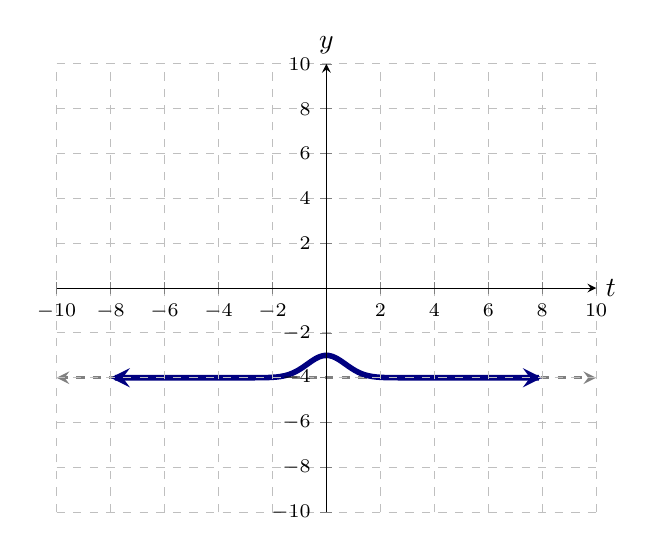
\begin{tikzpicture}
  \begin{axis}[
            domain=-10:10, ymax=10, xmax=10, ymin=-10, xmin=-10,
            axis lines =center, xlabel=$t$, ylabel={$y$}, grid = major, grid style={dashed},
            ytick={-10,-8,-6,-4,-2,2,4,6,8,10},
            xtick={-10,-8,-6,-4,-2,2,4,6,8,10},
            yticklabels={$-10$,$-8$,$-6$,$-4$,$-2$,$2$,$4$,$6$,$8$,$10$}, 
            xticklabels={$-10$,$-8$,$-6$,$-4$,$-2$,$2$,$4$,$6$,$8$,$10$},
            ticklabel style={font=\scriptsize},
            every axis y label/.style={at=(current axis.above origin),anchor=south},
            every axis x label/.style={at=(current axis.right of origin),anchor=west},
            axis on top
          ]
          
          \addplot [line width=1, gray, dashed,samples=100,domain=(-10:10),<->] {-4};

          %\addplot [line width=2, penColor2, smooth,samples=100,domain=(-6:2)] {-2*x-3};
          \addplot [line width=2, penColor, smooth,samples=100,domain=(-8:8),<->] {2.718^(-(x^2)) - 4};


  \end{axis}
\end{tikzpicture}
\end{image}





$g$ increases on $\left( -\infty, \answer{0} \right]$ and decreases on $\left[ \answer{0}, \infty \right)$.  This gives a global (also a local) maximum of $\answer{-3}$, which occurs at $\answer{0}$.   There are no minimums.


$\blacktriangleright$  $\answer{0}$ is the only critical number, because of the single extreme value.


$\blacktriangleright$  $g$ is continuous.  $\answer{-3}$ is a global maximum and the only extreme value. The end-behavior is that the function approaches $-4$. This gives a range of $\left( \answer{-4}, \answer{-3} \right]$.



\end{example}






$\blacktriangleright$ \textbf{\textcolor{red!80!black}{Notice:}}  The analysis was not simply graphing and describing the graph.  We don't trust graphs that much!  We want algebraic reasoning.  We want exact descriptions and the algebraic and function reasoning behind it.

We are not interested in a Visual Calculus course.  We are interested in an Algebraic Calculus course.  We want algebraic and function reasoning.  We want to know why conclusions are correct.

\textbf{\textcolor{red!80!black}{$\blacktriangleright$}} ``The graph looks like'' is not reassuring reasoning. 







\section*{with Calculus}

Calculus will give us the derivative $g'(t) = e^{-t^2} \cdot (-2t)$.  We could then solve $g'(t) = 0$ and verify that the only critical number is $t = 0$.












\begin{center}
\textbf{\textcolor{green!50!black}{ooooo-=-=-=-ooOoo-=-=-=-ooooo}} \\

more examples can be found by following this link\\ \link[More Examples of Analyzing More Functions]{https://ximera.osu.edu/csccmathematics/precalculus2/precalculus2/analyzingMoreFunctions/examples/exampleList}

\end{center}




\end{document}
